\documentclass[a4paper,11pt]{article}

\usepackage[margin=1in]{geometry}
\usepackage{amsmath,amssymb,amsthm,mathtools}
\usepackage{bm}
\usepackage{booktabs,array}
\usepackage{enumitem}
\usepackage{microtype}
\usepackage[dvipsnames]{xcolor}
\usepackage{tikz}
\usetikzlibrary{calc,positioning}
\usepackage[colorlinks=true,linkcolor=MidnightBlue,urlcolor=MidnightBlue]{hyperref}
\hypersetup{
  pdftitle={Hidden Region Finder}
}

\newcommand{\x}{\boldsymbol{x}}
\newcommand{\s}{\boldsymbol{s}}
\newcommand{\K}{\mathcal K}
\newcommand{\HR}{\mathrm{HR}}
\newcommand{\SL}{\mathrm{SL}}
\newcommand{\Obs}{\mathrm{Obs}}
\newcommand{\FSL}{\mathcal F_{\rm SL}}
\newcommand{\SSL}{\mathcal S_{\rm SL}}
\newcommand{\FObs}{\mathcal F_{\rm Obs}}
\newcommand{\WSL}{W_{\rm SL}}
\newcommand{\WHR}{W_{\rm HR}}
\newcommand{\vHR}{\vec v_{\rm HR}}
\newcommand{\Rpos}{\mathbb R_{>0}}
\newcommand{\ideal}{\mathcal I}
\newcommand{\dd}{\mathrm d}
\newcommand{\SLcolour}[1]{{\color{red}#1}}
\newcommand{\HRcolour}[1]{{\color{blue}#1}}
\newcommand{\Othercolour}[1]{{\color{black}#1}}

\tikzset{
 hrf internal/.style={thick},
 hrf contracted/.style={thick,densely dashed,red},
 hrf vertex/.style={circle,fill=black,draw=black,minimum size=3.2pt,
                    inner sep=0pt,outer sep=0pt},
 hrf edge label/.style={fill=white,inner sep=1pt,font=\scriptsize},
 hrf leg label/.style={font=\small}
}

\newtheorem{principle}{Principle}
\newtheorem{remark}{Remark}

\title{\bfseries Hidden Region Finder}
\author{}
\date{Working draft, 24 July 2026}

\begin{document}
\maketitle

\begin{abstract}
Hidden regions are contributions to asymptotic expansions that are invisible
to the ordinary Newton-polytope formulation of the Method of Regions because
nominally leading monomials cancel on a positive Landau pinch.  We introduce
the Hidden Region Finder (HRF), a parameter-space construction that determines
the cancellation locus, the superleading and obstruction polynomials, the
region scaling and the resolved leading Lee--Pomeransky polynomial.  It
handles general polynomial cancellation ideals, contraction-boundary
regions, asymptotic-order alignment and successive cancellation layers.  We
develop the construction for massless internal propagators, where the
Symanzik polynomials are linear in every individual Schwinger parameter.

Applications reveal a sparse topology-based organization that is not apparent
from individual region searches.  In the audited on-shell four-point sample
through four loops, every certified wide-angle or three-channel Regge hidden
region is associated with the three-loop Crown, either in the graph interior
or as a contraction minor; an exhaustive analysis of 16 mixed-sign four-loop
topologies without a Crown minor finds none.  These results support both the
Crown-minor and wide-angle-to-Regge conjectures in this sample.  In
addition, the five-loop SuperCrown supplies a positive contraction-minor test
beyond the four-loop audit.  In five-point spacelike-collinear scattering, a two-loop seed and its
vertex-corrected descendant show how an obstruction fixes a non-uniform
scaling and why genuinely non-binomial cancellation factors are required.
At six points, asymptotic-order alignment exposes a common positive
cancellation hypersurface for NMRK with \(w=z\) and for the double
spacelike-collinear limit.  The two expansions share the same factorized
superleading support but resolve it at different cancellation depths, and
therefore have distinct region vectors.  Thus HRF is not only a region-finding
algorithm: it exposes seed topologies and relations between kinematic
expansions.
\end{abstract}

\tableofcontents

\section{Introduction}

The Method of Regions (MoR) constructs the asymptotic expansion of a
multiscale Feynman integral as a sum of integrals associated with distinct
scalings of the integration variables.  Its geometric formulation in
parameter space maps every monomial of the Lee--Pomeransky polynomial to an
exponent point.  Lower facets of the resulting Newton polytope determine the
ordinary endpoint regions and their scaling vectors.

The Newton polytope retains the monomial exponents but not the information
carried by their coefficients.  In a physical Minkowski region, monomials of
opposite sign can cancel at positive values of the parameters.  If the
cancellation is reinforced by a Landau pinch, a set of monomials may be
individually more singular than the physical leading contribution while
their sum is suppressed.  The corresponding scaling is not a lower-facet
normal of the original polynomial and is therefore hidden from the ordinary
geometric construction.  We call it a \emph{hidden region} (HR).

A hidden region is specified by more than a scaling vector.  One must
identify the common positive cancellation locus, determine which monomials
form the superleading sector, resolve their cancellation against the
remaining Lee--Pomeransky polynomial, and verify that the resulting leading
integral is scaleful.  The Hidden Region Finder (HRF) is the systematic
parameter-space construction that performs these tasks.

The present paper concerns massless internal propagators only.  This is a
structural restriction, not a choice of examples: both Symanzik polynomials
are then multiaffine, or equivalently linear in every individual edge
parameter.  Internal masses add
\(\mathcal U\sum_e m_e^2x_e\) to \(\mathcal F\), which can generate
quadratic dependence on an individual \(x_e\).  Hidden regions in that more
general setting are important, but require a separate extension of the
construction and will not be treated here.

The presentation has two parts.  Part~I defines the construction without
reference to a particular graph.  Part~II develops the same ideas through a
sequence of massless examples.  Each example introduces one additional
phenomenon: a factorised cancellation with uniform scaling; an obstruction
that fixes a non-uniform scaling; non-binomial cancellation factors; and
finally composite limits for which preliminary asymptotic-order alignment and more than one
cancellation layer are required.

\part{Parameter-space formulation}

\section{Parametric representation and notation}
\label{sec:notation}

Consider a graph \(\mathcal G\) with \(N\) massless internal propagators and Lee--Pomeransky
(LP) polynomial
\begin{equation}
  \mathcal P(\x,\s)=\mathcal U(\x)+\mathcal F(\x;\s).
\end{equation}
The spanning-tree and spanning-2-forest formulae make the relevant structure
immediate.  For an \(L\)-loop graph, \(\mathcal U\) is homogeneous of degree
\(L\), while \(\mathcal F\) is homogeneous of degree \(L+1\) in the edge
parameters.  Each edge occurs at most once in every complementary
tree or 2-forest product.  Hence, for massless internal propagators, both
graph polynomials are linear in each individual \(x_e\).  This
multiaffinity is a standing assumption below.
Up to a normalisation which is irrelevant here, its integral has the form
\begin{equation}
 I_{\mathcal G}
 =
 \mathcal N_{\rm LP}
 \int_0^\infty
 \prod_{e=1}^{N}\frac{\dd x_e}{x_e}\,x_e^{\nu_e}\,
 \mathcal P(\x,\s)^{-D/2}.
\label{eq:LP}
\end{equation}
The \(N\) variables \(x_e\) are independent Lee--Pomeransky edge parameters,
each integrated over \((0,\infty)\).  In particular, there is no constraint
on \(\sum_e x_e\), or on the sum of any subset of the parameters.  We use
\(x_e\) rather than the conventional Feynman-parameter symbol \(\alpha_e\).

An optional, distinct projective representation can be obtained by
introducing one additional parameter \(x_0\) and the homogeneous polynomial
\begin{equation}
 \widehat{\mathcal P}(x_0,\x;\s)
 =\mathcal F(\x;\s)+x_0\mathcal U(\x).
\label{eq:homogenised-LP}
\end{equation}
There are then \(N+1\) parameters, and their common rescaling may be fixed by
inserting \(\delta(1-E(x_0,\x))\) for any positive degree-one homogeneous
function \(E\).  This homogenised embedding is distinct from the
non-projective LP integration space in \eqref{eq:LP} and is not assumed here.

Let \(\delta\to0^+\) define the kinematic expansion, and let \(\s\) denote a
set of real kinematic coordinates.  No sign convention is imposed on the
individual components of \(\s\); a physical domain \(\K\) is specified by
the appropriate inequalities among them.  This allows the same variables to
be retained across different physical regions, making changes of sign under
crossing or analytic continuation explicit.  A separate positive
parametrisation of a particular domain may be introduced locally as a
bookkeeping aid for proving inequalities or performing semialgebraic sign
tests, but neither the Newton-polytope construction nor the first-sheet pinch
condition requires it.  Retaining signed common variables also makes a
change in the existence of a cancellation directly visible in a factorised
superleading polynomial.  After expanding the kinematics, write
\begin{equation}
 \mathcal P(\x,\delta;\s)
 =
 \sum_i m_i,
 \qquad
 m_i\equiv
 c_i(\s)\,
 \delta^{a_i}\x^{\boldsymbol r_i},
 \qquad
 \x^{\boldsymbol r_i}
 =\prod_{e=1}^{N}x_e^{r_{i,e}}.
\label{eq:Pmonomials}
\end{equation}
Thus
\(\boldsymbol r_i=(r_{i,1},\ldots,r_{i,N})\) is the length-\(N\)
LP-parameter exponent vector of the monomial \(m_i\), while its augmented
length-\(N+1\) exponent point is
\begin{equation}
 \vec r_i=(\boldsymbol r_i;a_i)\in\mathbb R^{N+1}.
\end{equation}
No fixed sign of \(m_i\) on the whole physical domain is assumed.  Although
\(\delta^{a_i}\x^{\boldsymbol r_i}>0\) for \(\delta>0\) and \(\x>0\), the
coefficient \(c_i(\s)\) may vanish and change sign within or between the
domains under comparison.  The same qualification applies if several literal monomials have
been grouped into a kinematic coefficient or polynomial term.
A region vector is represented by an augmented normal whose last component
is normalised to one,
\begin{equation}
 \vec v_R=(\boldsymbol v_R;1),
 \qquad
 x_e\longmapsto \delta^{v_{R,e}}x_e,
\label{eq:regionvector}
\end{equation}
and the weight of a monomial is
\begin{equation}
 w_R(m_i)=\vec v_R\cdot\vec r_i
 =a_i+\boldsymbol v_R\cdot\boldsymbol r_i.
\label{eq:weight}
\end{equation}
The last component is always displayed when a vector is meant to be a
normal in augmented exponent space.  A list containing only the first \(N\)
entries is an LP-parameter scaling and not a fully normalised augmented
normal.

For a cancellation-free polynomial, the monomials of minimum weight form a
lower face of its Newton polytope.  A codimension-one lower face has an
inward-pointing normal whose last component is positive; after normalising
that component to one, the normal gives the corresponding facet-region
scaling.

\section{Hidden regions and positive pinches}
\label{sec:pinch}

The LP variables are integrated on the positive contour
\(\mathcal C_{\rm LP}=\mathbb R_{>0}^{N}\).  An interior first-sheet pinch of
a polynomial \(\mathcal Q(\x;\s)\) is therefore a solution
\begin{equation}
 \mathcal Q=0,
 \qquad
 \frac{\partial\mathcal Q}{\partial x_e}=0
 \quad(e=1,\ldots,N),
 \qquad
 \x\in\mathbb R_{>0}^{N},\quad \s\in\K.
\label{eq:positive-pinch}
\end{equation}
For a homogeneous polynomial, the derivative equations imply
\(\mathcal Q=0\) by Euler's identity.  On a contraction stratum the same
equations are imposed only on the active, nonzero parameters.

A cancellation in the positive orthant requires terms of both signs.
Consequently, every active derivative at an interior pinch must either vanish
identically or contain terms of both signs.  This elementary necessary
condition is useful as a rapid prefilter, but it neither identifies the
common pinch locus nor proves that a hidden region exists.  The defining
conditions below first use the scaling law to isolate \(\FSL\), and then
require a simultaneous positive solution of its derivative equations.

\section{Definition of a hidden region}
\label{sec:definition}

A HR is characterised by a superleading monomial support \(\SSL\), its
associated polynomial
\begin{equation}
 \FSL=\sum_{i\in\SSL}m_i,
\label{eq:FSLsupport}
\end{equation}
and a final scaling
\begin{equation}
 \vHR=(\boldsymbol v_{\HR};1)
\end{equation}
such that:
\begin{enumerate}[label=(\alph*)]
\item every monomial indexed by \(i\in\SSL\) has the same individual weight,
      \begin{equation}
        w_{\HR}(m_i)=\WSL,
        \qquad i\in\SSL;
      \label{eq:SLhomogeneity}
      \end{equation}
\item \(\FSL\) has a common first-sheet pinch in \(\K\),
      \begin{equation}
       \left.
       \frac{\partial\FSL}{\partial x_e}
       \right|_{\x>0,\,\s\in\K}=0
       \qquad\text{for every active }x_e;
      \label{eq:SLpinch}
      \end{equation}
\item the cancellation suppresses the sum of the superleading monomials to
      the first nonvanishing LP layer of weight \(\WHR\), with
      \begin{equation}
        \WHR>\WSL;
      \label{eq:gap}
      \end{equation}
\item after resolving the cancellation, the leading LP polynomial defines a
      scaleful lower-facet region.
\end{enumerate}
The gap \(\WHR-\WSL\) measures the depth of the cancellation.  It is a
physical output of the full problem and is not a freely chosen normalisation.

The superleading sector is not defined merely by mixed signs.  Mixed signs
are necessary for an interior pinch, but the simultaneous positive solution,
the hierarchy, and the final lower-facet condition are all essential.

\begin{principle}[Scaling precedes the positive pinch test]
The mixed-sign test is applied to derivatives of the starting polynomial
\(\mathcal F_\star\), but the simultaneous Landau equations are not.  The
weight homogeneity and separation conditions must first isolate the support
\(\SSL\).  The positive first-sheet equations are then imposed on the
resulting polynomial \(\FSL\).  Generically
\(\partial\mathcal F_\star/\partial x_e=0\) has no simultaneous positive
solution because \(\mathcal F_\star\) still contains the obstruction and
other terms excluded by the HR scaling.
\label{pr:scaling-before-pinch}
\end{principle}

\section{Cancellation ideals and the obstruction}
\label{sec:ordinary}

Before any LP-parameter scaling, expand
\begin{equation}
 \mathcal F(\x,\delta;\s)
 =
 \mathcal F_0(\x;\s)
 +\sum_{n>0}\delta^n\mathcal F_n(\x;\s).
\label{eq:Fexpansion}
\end{equation}
When the relevant superleading monomials are contained in
\(\mathcal F_0\), the cancellation analysis begins with
\(\mathcal F_\star=\mathcal F_0\).

\subsection{Cancellation factors and their common locus}

The derivatives of \(\mathcal F_\star\) are inspected for primitive,
non-monomial polynomial factors \(f_j(\x,\s)\) which can vanish for
\(\x>0\) and \(\s\in\K\).  At fixed \(\s\in\K\), a necessary condition
for such a zero is that the nonzero coefficients of the LP-parameter
monomials are not all of the same sign.  A
monomial factor such as \(x_e\) is not a cancellation hypersurface in the
interior and is removed from the primitive factor.

This inspection generates candidate cancellation structures; it is not a
Landau test on \(\mathcal F_\star\).  In particular, the full derivative
system of \(\mathcal F_\star\) is not required to have a positive solution at
this stage and generically does not.  A proposed relative scaling must first
select a homogeneous superleading support \(\SSL\) and strictly separate it
from the obstruction and all other monomials.

Only for the selected polynomial \(\FSL\) is the simultaneous first-sheet
pinch condition imposed.  When its derivative equations reduce to a set of
primitive cancellation factors, physical admissibility requires a common
positive zero at one and the same kinematic point:
\begin{equation}
 \exists\,(\x,\s)\in\Rpos^N\times\K:
 \qquad f_1(\x,\s)=\cdots=f_r(\x,\s)=0.
\label{eq:commonzero}
\end{equation}
Equivalently one solves \eqref{eq:SLpinch} directly.  The common locus,
rather than any one factor in isolation, encodes the pinch.  The elementary
mixed-sign condition can discard impossible ingredients, but it cannot
replace the scaling selection of \(\SSL\) or the subsequent simultaneous
positive solution.

\subsection{Generators and the obstruction decomposition}

Candidate generators are products of genuine cancellation polynomials,
\begin{equation}
 g_k=\prod_{f_j\in S_k}f_j,
\end{equation}
with at least two cancellation factors in the generator structures used by
HRF.  The factors, not monomial edge parameters, define the singular
hypersurfaces.  For a generator set \(G=\{g_1,\ldots,g_r\}\), define
\begin{equation}
 \mathcal I_{\rm canc}(G)
 =
 \langle g_1,\ldots,g_r\rangle.
\end{equation}
The HRF seeks a decomposition
\begin{equation}
 \mathcal F_\star=\FSL+\FObs,
 \qquad
 \FSL\in\mathcal I_{\rm canc}(G),
\label{eq:obstruction}
\end{equation}
or equivalently
\begin{equation}
 \FSL=\sum_kM_k(\x,\s)g_k.
\label{eq:idealpresentation}
\end{equation}
The polynomial \(\FObs\) is the obstruction: it prevents the full starting
polynomial from vanishing on the candidate cancellation locus but is to be
suppressed relative to the individual SL monomials by the HR scaling.

Different generator presentations can describe the same ideal and the same
pinch locus.  The presentation is a discovery device and does not label a
physical region.  Polynomial multipliers \(M_k\) in
\eqref{eq:idealpresentation} are allowed; a special factorised presentation
valid for one topology must not be promoted to a general rejection rule.

\section{Asymptotic-order alignment: selecting the correct starting face}
\label{sec:alignment}

\subsection{Why \texorpdfstring{\(\mathcal F_0\)}{F0} need not be the correct starting point}

In a composite limit, the relevant cancellation structure may not be visible
in the naive fixed-\(\x\) leading polynomial \(\mathcal F_0\).  A preliminary
LP-parameter rescaling can expose a different face of the full
\(\delta\)-dependent polynomial before the cancellation decomposition is
applied.  This operation is called \emph{asymptotic-order alignment}.

The rescaling changes the effective expansion order of a monomial from
\(a_i\) to \(a_i+\boldsymbol\phi\cdot\boldsymbol r_i\).  Monomials that
belong to different fixed-\(\x\) orders in \(\delta\) can thereby acquire a
common effective weight and enter the same cancellation sector.  This
cross-order alignment, rather than the mere selection of a different face,
is the purpose of the operation.

Let \(\boldsymbol\phi\in\mathbb Q^N\) be the preliminary alignment vector and define
\begin{equation}
 \omega_{\phi}(m_i)
 =
 a_i+\boldsymbol\phi\cdot\boldsymbol r_i.
\end{equation}
The order-aligned starting polynomial is the exposed face
\begin{equation}
 \mathcal F^{[\phi]}
 =
 \sum_{\substack{m_i\in\mathcal F\\
                  \omega_\phi(m_i)=
                  \min_{m_j\in\mathcal F}\omega_\phi(m_j)}}m_i.
\label{eq:alignmentface}
\end{equation}
The general HRF starting object is therefore
\begin{equation}
 \mathcal F_\star=
 \begin{cases}
   \mathcal F_0, & \text{ordinary search},\\
   \mathcal F^{[\phi]}, & \text{order-aligned search}.
 \end{cases}
\label{eq:Fstar}
\end{equation}
The same cancellation-factor, positive-pinch and obstruction analysis is
then applied to \(\mathcal F_\star\).

Asymptotic-order alignment is not itself the hidden-region scaling.  It
exposes the polynomial on which monomials from different original
\(\delta\)-orders can participate in one cancellation.  The HRF analysis of
that aligned face determines a cancellation ideal and a relative scaling
direction, but the final \(\vHR\) must still be determined from the complete
LP polynomial.

\subsection{Uniform-shift ambiguity}

The second Symanzik polynomial is homogeneous of fixed parameter degree.
Consequently,
\begin{equation}
 \boldsymbol\phi\longmapsto
 \boldsymbol\phi+c(1,\ldots,1)
\label{eq:uniformshift}
\end{equation}
adds the same amount to the weight of every monomial of \(\mathcal F\) and
does not change the face \(\mathcal F^{[\phi]}\).  The preliminary alignment
vector is therefore an equivalence class, not a unique vector.

This harmless ambiguity becomes important when \(\mathcal U\) is restored:
\(\mathcal U\) and \(\mathcal F\) have different parameter degrees, so the
shift changes their relative weights.  If \(\boldsymbol\rho\) denotes the
relative scaling returned by an HRF analysis of the selected face, the raw
sum
\begin{equation}
 \boldsymbol\phi+\boldsymbol\rho
\end{equation}
is not, in general, a shift-covariant definition of the physical total
vector.  It is a candidate presentation only.  The complete LP polynomial,
including \(\mathcal U\) and all occupied \(\delta\)-layers, must fix both the
uniform representative and the physical gap \(\WHR-\WSL\).

\section{Successive cancellation layers and the final vector}
\label{sec:layers}

\subsection{The complete LP polynomial is decisive}

For a candidate final vector, organise the complete polynomial into its
actually occupied weight layers,
\begin{equation}
 \mathcal P(\delta^{\boldsymbol v}\x,\delta;\s)
 =
 \sum_{q\in\Lambda}
 \delta^q\,\mathcal P_q(\x,\s),
\label{eq:weightlayers}
\end{equation}
where \(\Lambda\) is the set of weights which occur.  One must not insert
fictitious intermediate layers.  For example, if a parametrisation produces
only even powers of the expansion parameter, the absence of an odd power is
not an additional cancellation.

Let
\begin{equation}
 \ideal=\langle f_1,\ldots,f_r\rangle
\label{eq:pinchideal}
\end{equation}
be the ideal generated by independent cancellation factors defining the
common pinch.  A layer \(\mathcal P_q\) which lies in \(\ideal\) vanishes on
the pinch; a layer in \(\ideal^m\) vanishes to at least \(m\)-th order in
transverse directions.  The relevant information is its leading nonzero
class in the filtration
\begin{equation}
 \ideal^m/\ideal^{m+1}.
\label{eq:Iadic}
\end{equation}

Locally, take transverse coordinates \(y_j=f_j\).  If the approach to the
common pinch scales as
\begin{equation}
 y_j\sim\delta^{\tau_j},
 \qquad \tau_j>0,
\label{eq:transverseweights}
\end{equation}
then a jet \(y_1^{\beta_1}\cdots y_r^{\beta_r}\) in the \(q\)-th occupied
layer has effective weight
\begin{equation}
 q+\sum_j\beta_j\tau_j.
\label{eq:effectiveweight}
\end{equation}
The first resolved nonvanishing contribution, after accounting for these
transverse weights and the \(\mathcal U\) balance, defines \(\WHR\).  It need
not be the first nominal obstruction layer.  A second or later layer may
also vanish on the same singular locus.

All independent transverse coordinates must be suppressed with positive
weights.  A solution which suppresses only a proper subset of the
cancellation factors does not certify the common pinch under consideration.
Likewise, an unresolved continuous family signals that the total scaling has
not yet been fixed and may correspond to a residual scaleless rescaling.

\subsection{Hierarchy conditions}

The final, normalised vector \(\vHR=(\boldsymbol v_{\HR};1)\) must first
satisfy
\begin{equation}
 w_{\HR}(m_i)=\WSL,
 \qquad m_i\in\FSL.
\label{eq:finalSL}
\end{equation}
For the general, layered problem, the remaining hierarchy is a condition on
the resolved jets rather than on the nominal weights of individual
monomials.  If \(y^{\boldsymbol\beta}h_{\boldsymbol\beta}\) is a nonzero
leading jet of an occupied layer \(\mathcal P_q\), then
\begin{equation}
 q+\boldsymbol\beta\cdot\boldsymbol\tau
 \geq\WHR>\WSL,
\label{eq:finalhierarchy}
\end{equation}
and equality must occur for at least one resolved contribution.  A nominal
layer with \(q<\WHR\) is therefore allowed only if its positive ideal order
supplies enough transverse suppression to satisfy
\eqref{eq:finalhierarchy}.  This is precisely how a second cancellation
layer can occur.

If no intermediate ideal-valued layer is present, every term outside
\(\FSL\) has zero transverse ideal order.  In that special case
\eqref{eq:finalhierarchy} reduces to the single-layer monomial condition
\begin{equation}
 w_{\HR}(m_i)\geq\WHR>\WSL,
 \qquad m_i\in\mathcal P\setminus\FSL.
\label{eq:single-layer-hierarchy}
\end{equation}
Equations \eqref{eq:finalSL}--\eqref{eq:finalhierarchy}, the positive
transverse weights, and the balance with \(\mathcal U\) determine the
physical cancellation depth and remove the uniform alignment ambiguity.

Terms suppressed at fixed LP parameters must be restored before this
test.  If a term from \(\mathcal F_n\), \(n>0\), is promoted to the SL level
or below by the candidate scaling, then the proposed \(\FSL\) is incomplete
and the analysis must be repeated with that term included.

\section{Scalefulness and dissection}
\label{sec:scaleful}

Whether the region integral is scaleful is a property of the resolved
monomial support of the LP polynomial.  It does not depend on the
space-time dimension \(D\).  A mere count of variables appearing in selected
monomials is a useful diagnostic but is not a general certificate.

After the cancellations are resolved, the decisive geometric requirement is
that the leading support define a lower facet with an inward-pointing normal
whose last component is positive.  There are two cases.

\begin{enumerate}[label=(\arabic*)]
\item If the monomials at the resolved \(\WHR\) layer already exhibit the
      required lower facet in the original coordinates, this is a sufficient
      certificate and no change of variables is needed.
\item If that test is inconclusive, or if the full-layer equations do not
      fix a unique total vector, one must use local coordinates adapted to
      the pinch.  A dissection separates the integration domain into sectors
      and maps the cancellation hypersurfaces to endpoints.  In each sector
      the polynomial is cancellation-free, so the ordinary Newton-polytope
      facet criterion is both the safe region test and the direct route to
      the region integral.
\end{enumerate}

The facet normal obtained after dissection is pulled back to the original
LP coordinates and then normalised with last component one.  This
pullback is the authoritative total vector.  It may differ from the raw
alignment-plus-relative-HRF sum because the latter retains the ambiguity described
in \eqref{eq:uniformshift} and may not have resolved all cancellation layers.

Dissection is therefore not required for every discovery.  A unique
ideal-layer solution supplies the same certification in the original
coordinates.  Dissection remains the necessary fallback when the local
ideal geometry is nonlinear, singular or non-unique, and it is often useful
later for evaluating the HR integral.

\section{Boundary hidden regions}
\label{sec:boundary}

An interior HR has all \(x_e>0\).  A boundary HR occurs on a contraction
stratum
\begin{equation}
 x_{e_1}=\cdots=x_{e_k}=0.
\end{equation}
The graph polynomial is first restricted to that stratum, the vanished
variables are removed, and the complete analysis is repeated with every
remaining active parameter positive.  In graph language this is the
corresponding contraction minor; in Landau language it is a subleading
Landau singularity.

A complete search must include the relevant contraction strata.  Failure to
find an interior HR is not a proof that the graph has no HR.

\section{When do two presentations describe the same HR?}
\label{sec:equivalence}

Generator lists are not physical labels.  Two presentations describe the
same HR when they determine the same physical component of the common pinch
locus, the same resolved leading facet, and the same pulled-back total
scaling vector.  Replacing a generator set by another presentation of the
same relevant ideal does not create a new region.

Genuinely distinct HRs can arise from:
\begin{itemize}
\item different positive components of the cancellation variety;
\item different cancellation ideals or singular hypersurface systems; or
\item different lower facets in local coordinates, and hence different
      certified pullback vectors.
\end{itemize}
Thus a raw multiplicity of accepted generator presentations must be reduced
by ideal, positive-locus and final-facet equivalence before being interpreted
as multiple physical HRs.

\section{Generator-independent certificates of absence}
\label{sec:absence}

Factor harvesting is efficient for discovery, but a definitive negative
statement should not depend on a maximum factor length, a maximum number of
generators or a preferred factorised presentation.

The homogeneity condition \eqref{eq:SLhomogeneity}, together with strict
separation from all non-SL monomials, implies that the exponent support of
\(\FSL\) is an exposed face of the appropriate starting support.  This gives
a generator-independent route:
\begin{enumerate}[label=\arabic*.]
\item enumerate every relevant exposed face of \(\mathcal F_0\), or of the
      augmented full support when asymptotic-order alignment is allowed;
\item interpret each face polynomial as a candidate \(\FSL\) selected by
      its face normal, and discard faces that fail elementary necessary
      conditions;
\item solve the simultaneous positive logarithmic Landau equations for every
      surviving candidate \(\FSL\) in \(\K\);
\item test each positive solution against \(\mathcal U\), every occupied
      restored \(\delta\)-layer, the hierarchy gap and the resolved lower
      facet;
\item repeat the analysis on all required contraction strata.
\end{enumerate}

If every face is excluded by one of these exact steps, there is no HR within
the stated first-sheet and asymptotic assumptions.  If a search limit,
timeout or undecided positivity question is reached, the result is
\emph{unresolved}, not evidence for absence.

\section{The Hidden Region Finder}
\label{sec:workflow}

The complete conceptual workflow is:
\begin{enumerate}[label=\textbf{\arabic*.},leftmargin=*]
\item \textbf{Fix the physical chart.}
      Specify \(\delta\to0^+\), a common set of real kinematic coordinates
      \(\s\), and the inequalities defining the physical domain \(\K\).
      Introduce positive coordinates only locally if they simplify a
      particular positivity test.
\item \textbf{Choose a stratum.}
      Start in the interior and repeat on the required contraction strata.
\item \textbf{Choose the starting face.}
      Use \(\mathcal F_0\) in the ordinary case; when necessary enumerate
      order-aligned exposed faces \(\mathcal F^{[\phi]}\) of the full
      \(\delta\)-dependent polynomial.
\item \textbf{Generate candidate cancellation structures.}
      Apply the mixed-sign test to the individual derivatives of
      \(\mathcal F_\star\) only as a necessary prefilter, and harvest
      primitive non-monomial factors and candidate generator structures.
      Do not solve the simultaneous derivative equations of
      \(\mathcal F_\star\): they generically have no positive solution.
\item \textbf{Isolate the superleading support by scaling.}
      Solve the homogeneous-weight and strict-separation conditions that
      select \(\SSL\) from the starting support.  Define
      \(\FSL=\sum_{i\in\SSL}m_i\), determine the candidate relative
      hierarchy, and decompose
      \(\mathcal F_\star=\FSL+\FObs\).  Retain every intermediate occupied
      layer for the full certification.
\item \textbf{Apply the first-sheet pinch test to \(\FSL\).}
      Only after \(\SSL\) has been isolated, solve
      \(\partial\FSL/\partial x_e=0\) simultaneously for all active
      parameters with \(\x>0\) and \(\s\in\K\).  The resulting common
      positive locus defines the physical cancellation ideal; reject the
      candidate if this system has no solution.
\item \textbf{Resolve all occupied cancellation layers.}
      Use the ideal filtration of the complete
      \(\mathcal P=\mathcal U+\mathcal F\), positive transverse weights and
      the actual \(\delta\)-weight lattice to find the first nonvanishing
      layer.
\item \textbf{Fix and certify the total vector.}
      Determine \(\vHR=(\boldsymbol v_{\HR};1)\), \(\WSL\), \(\WHR\) and the
      gap.  Certify the lower facet in original coordinates when possible;
      otherwise dissect and pull the facet normal back.
\item \textbf{Identify physical equivalence classes.}
      Merge generator presentations that describe the same positive pinch
      component and final facet.
\item \textbf{State completeness honestly.}
      A positive HR requires all certification stages.  A no-HR conclusion
      requires exhaustive face and boundary coverage; incomplete searches
      remain unresolved.
\end{enumerate}

\part{Examples}

\section{How to read the colour-coded polynomials}
\label{sec:example-colours}

Every example will display the relevant part of \(\mathcal F\) using one
colour convention.  The colours refer to weights under the \emph{final total
region vector}; in a composite limit this includes both the preliminary
asymptotic-order alignment and the relative HRF scaling:
\begin{equation}
 \boxed{\begin{aligned}
 \SLcolour{\text{red}}\;&=\text{individually superleading terms at }\WSL,\\
 \HRcolour{\text{blue}}\;&=\text{resolved leading terms at }\WHR,\\
 \Othercolour{\text{black}}\;&=\text{all other terms}.
 \end{aligned}}
\label{eq:colour-key}
\end{equation}
Thus a conventional facet region contains blue leading terms and black
subleading terms, but no red sector.  In a hidden region the red monomials
have a lower individual weight than the blue monomials, but their sum
vanishes on the positive pinch.  The blue terms therefore give the actual
leading polynomial.  Black also includes any intermediate layer that lies
in the cancellation ideal and vanishes before the blue layer is reached.

Schematically, the comparison is
\begin{align}
 \mathcal F^{(R)}
 &=\delta^{W_R}\HRcolour{\mathcal F_{W_R}}
   +\Othercolour{\mathcal O(\delta^{>W_R})},
 &&\text{ordinary facet region},
\label{eq:facet-colour-schematic}\\
 \mathcal F^{(\HR)}
 &=\delta^{\WSL}\SLcolour{\FSL}
   +\delta^{\WHR}\HRcolour{\mathcal F_{\HR}}
   +\Othercolour{\mathcal O(\delta^{>\WHR})},
 &&\text{hidden region},
\label{eq:HR-colour-schematic}
\end{align}
where the first term in \eqref{eq:HR-colour-schematic} vanishes on the pinch.
This is a classification of the terms, not an instruction to discard the
red polynomial before the cancellation has been established.

Every family below is presented in the same order:
\begin{enumerate}[label=(\roman*)]
 \item the kinematic expansion and its physical domain;
 \item the graph and the assignment of Schwinger parameters;
 \item the decomposition \(\mathcal F_\star=\FSL+\FObs\) and its positive
 cancellation locus;
 \item the certified total vector \((\boldsymbol v;1)\), including
 \((\WSL,\WHR)\);
 \item the feature that the algorithm must retain in order not to miss the
 region.
\end{enumerate}
The examples are therefore a tour through possible HR mechanisms, rather
than a chronology of how the implementation was developed.

\section{The Crown family: an interior seed and its contraction descendants}
\label{sec:example-crown}

\subsection{Wide-angle kinematics and the three-loop seed}

Take four external momenta in the physical \(2\to2\) domain
\begin{equation}
 s_{12}>0,\qquad s_{23}<0,\qquad s_{12}>-s_{23},
 \label{eq:crown-domain}
\end{equation}
and regulate the on-shell limit by \(p_i^2=\delta q_i^2\), with fixed
nonzero \(q_i^2\) and \(\delta\to0^+\).  A common normalization of the
\(q_i^2\) is immaterial for the region vector.  The Crown has internal edge
set
\begin{equation}
 \begin{split}
 E_C={}&\{(1,5),(1,6),(2,5),(2,6),\\[-1mm]
       &\hspace{18mm}(3,5),(3,6),(4,5),(4,6)\},
 \end{split}
 \label{eq:crown-edges}
\end{equation}
in the order \(x_1,\ldots,x_8\), with \(p_i\) attached to vertex \(i\) for
\(i=1,\ldots,4\).  This edge list fixes the graph without relying on a
particular drawing.

\begin{figure}[htbp]
\centering
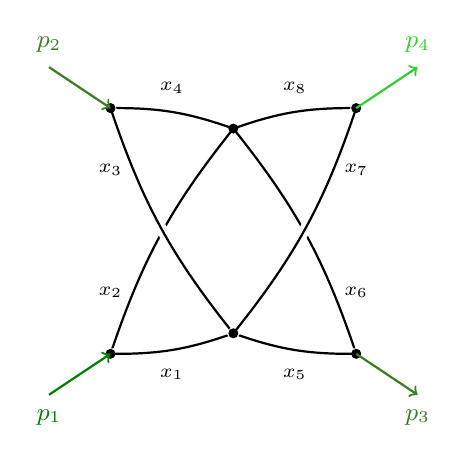
\begin{tikzpicture}[scale=.52]
 \coordinate (v1) at (2,2);
 \coordinate (v2) at (2,8);
 \coordinate (v3) at (8,2);
 \coordinate (v4) at (8,8);
 \coordinate (v5) at (5,2.5);
 \coordinate (v6) at (5,7.5);

 % Square embedding used in the original wide-angle analysis.
 \draw[hrf internal] (v6) to[bend right=10] (v1);
 \draw[hrf internal] (v6) to[bend right=10] (v2);
 \draw[hrf internal] (v6) to[bend left=10] (v3);
 \draw[hrf internal] (v6) to[bend left=10] (v4);
 % White underlays distinguish crossings from vertices.
 \foreach \a/\b/\bend in {v5/v1/left,v5/v2/left,v5/v3/right,v5/v4/right}{
   \draw[white,line width=4pt] (\a) to[bend \bend=10] (\b);
   \draw[hrf internal] (\a) to[bend \bend=10] (\b);
 }

 \node[hrf edge label] at (3.5,1.5) {$x_1$};
 \node[hrf edge label] at (2,3.5) {$x_2$};
 \node[hrf edge label] at (2,6.5) {$x_3$};
 \node[hrf edge label] at (3.5,8.5) {$x_4$};
 \node[hrf edge label] at (6.5,1.5) {$x_5$};
 \node[hrf edge label] at (8,3.5) {$x_6$};
 \node[hrf edge label] at (8,6.5) {$x_7$};
 \node[hrf edge label] at (6.5,8.5) {$x_8$};

 \foreach \v in {1,...,6} \node[hrf vertex] at (v\v) {};
 \draw[->,thick,Green] (.5,1)--(v1);
 \draw[->,thick,OliveGreen] (.5,9)--(v2);
 \draw[->,thick,OliveGreen] (v3)--(9.5,1);
 \draw[->,thick,LimeGreen] (v4)--(9.5,9);
 \node[hrf leg label,text=Green] at (.5,.45) {$p_1$};
 \node[hrf leg label,text=OliveGreen] at (.5,9.55) {$p_2$};
 \node[hrf leg label,text=OliveGreen] at (9.5,.45) {$p_3$};
 \node[hrf leg label,text=LimeGreen] at (9.5,9.55) {$p_4$};
\end{tikzpicture}
\caption{The three-loop Crown with the Schwinger-parameter assignment used in
Eq.~\eqref{eq:crown-edges}.  The external-arrow colours are visual label
guides only.}
\label{fig:crown-graph}
\end{figure}

At fixed parameters the leading polynomial is
\begin{align}
 \mathcal F_0={}&
 \SLcolour{s_{12}(x_4x_5-x_3x_6)(x_2x_7-x_1x_8)}
 \nonumber\\[-2mm]
 &\hspace{22mm}
 \SLcolour{-s_{23}(x_2x_3-x_1x_4)(x_6x_7-x_5x_8)}.
 \label{eq:crown-F0}
\end{align}
The four displayed binomials vanish on one common positive component; only
three equations are independent there.  Hence
\begin{equation}
 \mathcal F_\star=\mathcal F_0=\FSL,
 \qquad \FObs=0.
 \label{eq:crown-no-obstruction}
\end{equation}
Writing \(\mathcal F=\mathcal F_0+\delta\mathcal F_1+\cdots\), the certified
vector and weights are
\begin{equation}
 \vHR=(-1,-1,-1,-1,-1,-1,-1,-1;1),
 \qquad (\WSL,\WHR)=(-4,-3).
 \label{eq:crown-vector}
\end{equation}
Consequently
\begin{equation}
 \mathcal P(\delta^{-1}\x,\delta)
 =\delta^{-4}\SLcolour{\mathcal F_0}
 +\delta^{-3}\HRcolour{\bigl(\mathcal F_1+\mathcal U\bigr)}
 +\Othercolour{\mathcal O(\delta^{-2})}.
 \label{eq:crown-colours}
\end{equation}
The algorithmic lesson is the most elementary one: HRF must keep a
simultaneous positive zero of several cancellation factors.  No obstruction,
non-uniform scaling or preliminary alignment is needed.

\subsection{The same seed in Regge limits}

Momentum conservation gives \(s_{13}=-s_{12}-s_{23}\).  The three channel
charts used in the audit are
\begin{align}
 T_{23}:&\quad s_{23}=-\delta s_{12}, &&s_{12}>0,\nonumber\\
 T_{12}:&\quad s_{12}=-\delta s_{23}, &&s_{23}<0,\nonumber\\
 T_{13}:&\quad s_{23}=-s_{12}+\delta s_{12}, &&s_{12}>0,
 \label{eq:crown-regge-charts}
\end{align}
with \(\delta\to0^+\).  The Crown HR is present in all three charts.  The
surviving cancellation equations are channel dependent, but they are
restrictions of the same wide-angle positive pinch.  This is the positive
seed for the observed wide-angle-to-Regge correspondence.

\subsection{SuperCrown and HyperCrown boundary regions}
\label{sec:example-crown-boundaries}

Higher-loop graphs inherit the seed on contraction strata.  In edge
order, the two graphs are
\begin{align}
E_{SC}={}&\{(1,5),(1,6),(2,7),(2,6),(3,5),(3,8),
 (4,7),(4,8),(5,7),(6,8),(7,8),(5,6)\},
\nonumber\\
E_{HC}={}&\{(1,5),(1,6),(4,9),(4,6),(2,7),(2,6),
 (3,8),(3,6),(9,5),(7,8),(8,9),(5,7)\}.
\label{eq:crown-descendant-edges}
\end{align}

\begin{figure}[htbp]
\centering
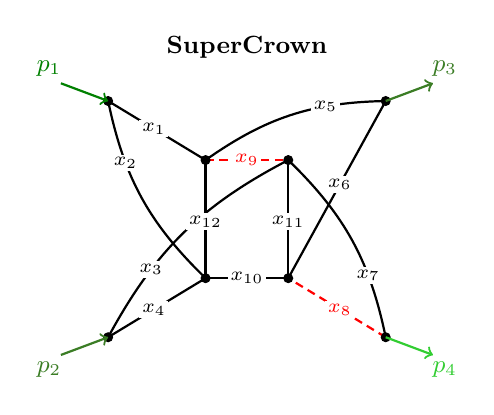
\begin{tikzpicture}[scale=.75]
 \coordinate (v1) at (-2.35,2.00);
 \coordinate (v2) at (-2.35,-2.00);
 \coordinate (v3) at (2.35,2.00);
 \coordinate (v4) at (2.35,-2.00);
 \coordinate (v5) at (-0.70,1.00);
 \coordinate (v6) at (-0.70,-1.00);
 \coordinate (v7) at (0.70,1.00);
 \coordinate (v8) at (0.70,-1.00);
 \node[font=\small\bfseries] at (0,2.90) {SuperCrown};

 \draw[hrf internal] (v1)--node[hrf edge label,pos=.47] {$x_1$}(v5);
 \draw[hrf internal] (v1) to[bend right=17]
   node[hrf edge label,pos=.30] {$x_2$}(v6);
 \draw[hrf internal] (v2) to[bend left=17]
   node[hrf edge label,pos=.30] {$x_3$}(v7);
 \draw[hrf internal] (v2)--node[hrf edge label,pos=.47] {$x_4$}(v6);
 \draw[hrf internal] (v3) to[bend right=17]
   node[hrf edge label,pos=.30] {$x_5$}(v5);
 \draw[hrf internal] (v3)--node[hrf edge label,pos=.47] {$x_6$}(v8);
 \draw[hrf internal] (v4) to[bend right=17]
   node[hrf edge label,pos=.30] {$x_7$}(v7);
 \draw[hrf contracted] (v4)--node[hrf edge label,pos=.47,text=red] {$x_8$}(v8);
 \draw[hrf contracted] (v5)--node[hrf edge label,pos=.50,text=red] {$x_9$}(v7);
 \draw[hrf internal] (v6)--node[hrf edge label,pos=.50] {$x_{10}$}(v8);
 \draw[hrf internal] (v7)--node[hrf edge label,pos=.52] {$x_{11}$}(v8);
 \draw[hrf internal] (v5)--node[hrf edge label,pos=.52] {$x_{12}$}(v6);

 \foreach \v in {1,...,8} \node[hrf vertex] at (v\v) {};
 \draw[->,thick,Green] (-3.15,2.30)--(v1);
 \draw[->,thick,OliveGreen] (-3.15,-2.30)--(v2);
 \draw[->,thick,OliveGreen] (v3)--(3.15,2.30);
 \draw[->,thick,LimeGreen] (v4)--(3.15,-2.30);
 \node[hrf leg label,text=Green] at (-3.35,2.55) {$p_1$};
 \node[hrf leg label,text=OliveGreen] at (-3.35,-2.55) {$p_2$};
 \node[hrf leg label,text=OliveGreen] at (3.35,2.55) {$p_3$};
 \node[hrf leg label,text=LimeGreen] at (3.35,-2.55) {$p_4$};
\end{tikzpicture}
\hspace{5mm}
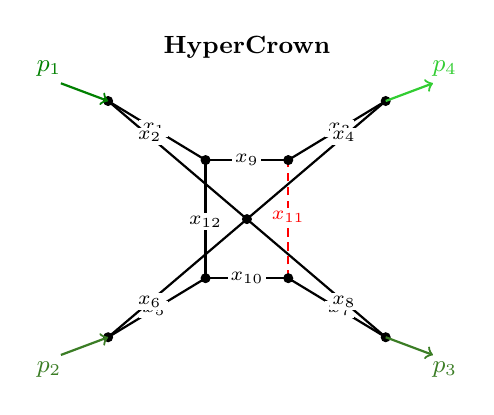
\begin{tikzpicture}[scale=.75]
 \coordinate (v1) at (-2.35,2.00);
 \coordinate (v2) at (-2.35,-2.00);
 \coordinate (v4) at (2.35,2.00);
 \coordinate (v3) at (2.35,-2.00);
 \coordinate (v5) at (-0.70,1.00);
 \coordinate (v9) at (0.70,1.00);
 \coordinate (v8) at (0.70,-1.00);
 \coordinate (v7) at (-0.70,-1.00);
 \coordinate (v6) at (0,0);
 \node[font=\small\bfseries] at (0,2.90) {HyperCrown};

 \draw[hrf internal] (v1)--node[hrf edge label,pos=.47] {$x_1$}(v5);
 \draw[hrf internal] (v1)--node[hrf edge label,pos=.30] {$x_2$}(v6);
 \draw[hrf internal] (v4)--node[hrf edge label,pos=.47] {$x_3$}(v9);
 \draw[hrf internal] (v4)--node[hrf edge label,pos=.30] {$x_4$}(v6);
 \draw[hrf internal] (v2)--node[hrf edge label,pos=.47] {$x_5$}(v7);
 \draw[hrf internal] (v2)--node[hrf edge label,pos=.30] {$x_6$}(v6);
 \draw[hrf internal] (v3)--node[hrf edge label,pos=.47] {$x_7$}(v8);
 \draw[hrf internal] (v3)--node[hrf edge label,pos=.30] {$x_8$}(v6);
 \draw[hrf internal] (v9)--node[hrf edge label,pos=.50] {$x_9$}(v5);
 \draw[hrf internal] (v7)--node[hrf edge label,pos=.50] {$x_{10}$}(v8);
 \draw[hrf contracted] (v8)--node[hrf edge label,pos=.52,text=red] {$x_{11}$}(v9);
 \draw[hrf internal] (v5)--node[hrf edge label,pos=.52] {$x_{12}$}(v7);

 \foreach \v in {1,...,9} \node[hrf vertex] at (v\v) {};
 \draw[->,thick,Green] (-3.15,2.30)--(v1);
 \draw[->,thick,OliveGreen] (-3.15,-2.30)--(v2);
 \draw[->,thick,OliveGreen] (v3)--(3.15,-2.30);
 \draw[->,thick,LimeGreen] (v4)--(3.15,2.30);
 \node[hrf leg label,text=Green] at (-3.35,2.55) {$p_1$};
 \node[hrf leg label,text=OliveGreen] at (-3.35,-2.55) {$p_2$};
 \node[hrf leg label,text=OliveGreen] at (3.35,-2.55) {$p_3$};
 \node[hrf leg label,text=LimeGreen] at (3.35,2.55) {$p_4$};
\end{tikzpicture}
\caption{Higher-loop Crown descendants: the five-loop SuperCrown (left) and
the four-loop HyperCrown (right).  Red dashed edges are set to zero on the
contraction strata used in the HR analysis: \(x_8=x_9=0\) for the SuperCrown
and \(x_{11}=0\) for the HyperCrown.}
\label{fig:crown-descendant-graphs}
\end{figure}

The SuperCrown stratum \(x_8=x_9=0\) and the HyperCrown stratum
\(x_{11}=0\) expose a Crown contraction minor.  On the surviving coordinates
the restricted polynomial has the decomposition
\begin{equation}
 \mathcal F_\star\big|_{\rm stratum}
 =\FSL^{C}+0,
 \qquad
 \boldsymbol v_{\rm surv}=(-1,\ldots,-1),
 \qquad (\WSL,\WHR)=(-4,-3),
 \label{eq:crown-descendant-data}
\end{equation}
up to graph-dependent monomial factors and relabelling.  The contracted
parameters are fixed to zero and are not entries of
\(\boldsymbol v_{\rm surv}\).  The SuperCrown region is certified at wide
angle and in all three Regge charts; the HyperCrown is certified at wide
angle and in the recorded \(T_{12}\) Regge chart.

This family adds two indispensable capabilities.  First, the search must
descend to boundary strata: an interior-only analysis misses a region that
is present in the parent integral.  Second, candidate generation in the
parent graphs must retain primitive polynomial derivative factors, including
non-binomial ones.  The relevant object is the ideal they generate after
restriction, not a preferred pairwise factorization of the full polynomial.

The converse audit completes the tested four-loop picture.  Sixteen
mixed-sign topologies without a Crown contraction minor have no certified
interior or boundary HR at wide angle or in any of the three Regge channels.
Thus the tested sample supports both the Crown-minor conjecture and the
wide-angle-to-Regge conjecture through four loops.  These are empirical
statements for the audited graphs, not general graph-theoretic theorems.

\section{Five-point spacelike-collinear scattering: obstruction and general polynomial factors}
\label{sec:example-five-point}

\subsection{Kinematics and the two-loop seed graph}

The collinear chart is defined by
\begin{equation}
 \begin{gathered}
 s_{12}=sz,\qquad s_{23}=-4\delta^2,\qquad
 s_{34}=-s\chi(z-1),\\
 s_{45}=s,\qquad s_{15}=s\chi+c\delta,\qquad \delta\to0^+,
 \end{gathered}
 \label{eq:five-kinematics}
\end{equation}
with
\begin{equation}
 s>0,\qquad z>1,\qquad -1<\chi<0,
 \label{eq:five-domain}
\end{equation}
and fixed nonzero \(c\).  Keeping \(\chi\) negative is useful: the same
variables then display directly the change from timelike to spacelike
collinear kinematics.

The two-loop seed has edge set
\begin{equation}
 E_5=\{(1,3),(1,5),(2,3),(2,5),(3,4),(4,5)\}
 \longleftrightarrow (x_1,\ldots,x_6),
 \label{eq:five-edges}
\end{equation}
and external attachment \(p_i\to i\), \(i=1,\ldots,5\).  We use
\(x_{i,j,\ldots}=x_ix_j\cdots\).

\begin{figure}[htbp]
\centering
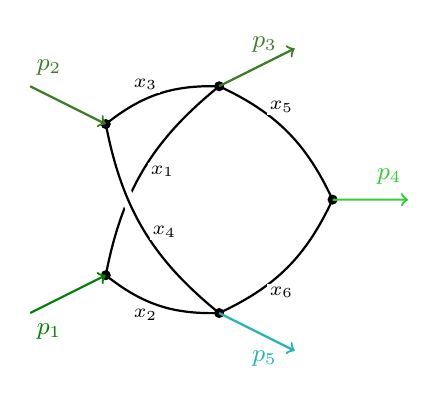
\begin{tikzpicture}[scale=.48]
 \coordinate (v1) at (2,3);
 \coordinate (v2) at (2,7);
 \coordinate (v3) at (5,8);
 \coordinate (v4) at (8,5);
 \coordinate (v5) at (5,2);

 \draw[hrf internal] (v3) to[bend right=20] (v1);
 \draw[hrf internal] (v3) to[bend right=20] (v2);
 \draw[white,double=white,double distance=3pt,thick]
   (v5) to[bend left=20] (v2);
 \draw[hrf internal] (v5) to[bend left=20] (v2);
 \draw[hrf internal] (v5) to[bend left=20] (v1);
 \draw[hrf internal] (v3) to[bend left=20] (v4);
 \draw[hrf internal] (v5) to[bend right=20] (v4);

 \foreach \v in {1,...,5} \node[hrf vertex] at (v\v) {};
 \draw[->,thick,Green] (0,2)--(v1);
 \draw[->,thick,OliveGreen] (0,8)--(v2);
 \draw[->,thick,OliveGreen] (v3)--(7,9);
 \draw[->,thick,LimeGreen] (v4)--(10,5);
 \draw[->,thick,TealBlue] (v5)--(7,1);

 \node[hrf leg label,text=Green] at (.5,1.5) {$p_1$};
 \node[hrf leg label,text=OliveGreen] at (.5,8.5) {$p_2$};
 \node[hrf leg label,text=OliveGreen] at (6.2,9.1) {$p_3$};
 \node[hrf leg label,text=LimeGreen] at (9.5,5.6) {$p_4$};
 \node[hrf leg label,text=TealBlue] at (6.2,.8) {$p_5$};

 \node[hrf edge label] at (3.50,5.75) {$x_1$};
 \node[hrf edge label] at (3.05,1.95) {$x_2$};
 \node[hrf edge label] at (3.05,8.05) {$x_3$};
 \node[hrf edge label] at (3.55,4.15) {$x_4$};
 \node[hrf edge label] at (6.65,7.45) {$x_5$};
 \node[hrf edge label] at (6.65,2.55) {$x_6$};
\end{tikzpicture}
\caption{The two-loop five-point seed graph, redrawn in the style of
Ref.~\cite{GardiEtAl2026}, with the Schwinger parameters used in
Eqs.~\eqref{eq:five-facet-F0}--\eqref{eq:five-HR-Fdelta}.}
\label{fig:five-point-seed}
\end{figure}

\subsection{One polynomial, an ordinary facet and a hidden region}

For the ordinary facet vector
\begin{equation}
 \vec v_C=(-2,0,-2,-2,-2,0;1),
 \label{eq:five-facet-vector}
\end{equation}
the expanded polynomial is classified as
\begin{align}
 \mathcal F_0^{[C]}={}&
 \HRcolour{s\bigl(x_{2,5}+\chi x_{1,6}\bigr)
       \bigl[(z-1)x_3-x_4\bigr]}
 +\Othercolour{sz(\chi+1)x_{2,3,6}},
 \label{eq:five-facet-F0}\\
 \mathcal F_\delta^{[C]}={}&
 \Othercolour{-c\delta x_{1,4,6}+c\delta x_{2,3,6}}
 +\HRcolour{4\delta^2x_{1,4,5}}
 \Othercolour{-4\delta^2x_{2,3,5}}.
 \label{eq:five-facet-Fdelta}
\end{align}
There is no red sector: the blue monomials form an ordinary lower facet.

For the hidden-region vector
\begin{equation}
 \vHR=(-2,-1,-2,-2,-2,-1;1),
 \qquad (\WSL,\WHR)=(-5,-4),
 \label{eq:five-HR-vector}
\end{equation}
the identical polynomial instead reads
\begin{align}
 \mathcal F_0^{[\HR]}={}&
 \underbrace{\SLcolour{s\bigl(x_{2,5}+\chi x_{1,6}\bigr)
       \bigl[(z-1)x_3-x_4\bigr]}}_{\FSL}
 +\underbrace{\HRcolour{sz(\chi+1)x_{2,3,6}}}_{\FObs},
 \label{eq:five-HR-F0}\\
 \mathcal F_\delta^{[\HR]}={}&
 \HRcolour{-c\delta x_{1,4,6}}
 +\Othercolour{c\delta x_{2,3,6}}
 +\HRcolour{4\delta^2x_{1,4,5}}
 \Othercolour{-4\delta^2x_{2,3,5}}.
 \label{eq:five-HR-Fdelta}
\end{align}
The cancellation ideal is generated by
\begin{equation}
 f_1=x_{2,5}+\chi x_{1,6},\qquad
 f_2=(z-1)x_3-x_4,\qquad \ideal=\langle f_1,f_2\rangle.
 \label{eq:five-generator}
\end{equation}
The red product vanishes at the positive pinch.  The blue obstruction,
the blue kinematically suppressed terms, and
\begin{equation}
 \mathcal U_{\WHR}
 =\HRcolour{x_{1,3}+x_{1,4}+x_{1,5}+x_{3,5}+x_{4,5}}
 \label{eq:five-U-leading}
\end{equation}
form the physical layer.  This example introduces the obstruction:
\(\FObs\ne0\) fixes a non-uniform scaling that would not be determined by
the factorized cancellation sector alone.

\subsection{The vertex-corrected graph: a genuinely non-binomial generator}

The same kinematics applied to the three-loop vertex-corrected graph gives
\begin{equation}
 \begin{split}
 E_{5V}={}&\{(1,3),(1,5),(3,7),(6,5),(3,4),\\[-1mm]
          &\hspace{17mm}(4,5),(2,7),(6,7),(2,6)\}
 \longleftrightarrow (x_0,\ldots,x_8).
 \end{split}
 \label{eq:five-vertex-edges}
\end{equation}

\begin{figure}[htbp]
\centering
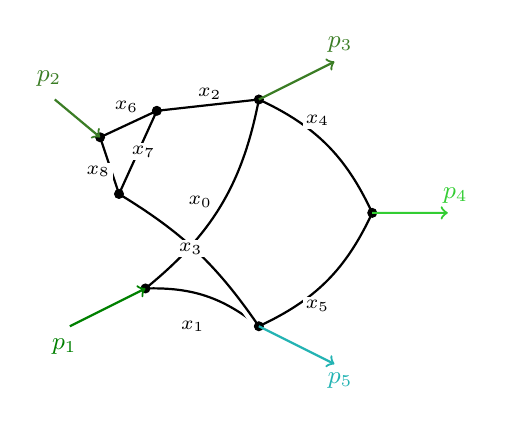
\begin{tikzpicture}[scale=.48]
 \coordinate (v1) at (2,3);
 \coordinate (v2) at (0.8,7);
 \coordinate (v3) at (5,8);
 \coordinate (v4) at (8,5);
 \coordinate (v5) at (5,2);
 \coordinate (v7) at (2.3,7.7);
 \coordinate (v6) at (1.3,5.5);

 \draw[hrf internal] (v1) to[bend right=20] (v3);
 \draw[hrf internal] (v1) to[bend left=20] (v5);
 \draw[hrf internal] (v3)--(v7);
 \draw[white,line width=4pt] (v6) to[bend left=12] (v5);
 \draw[hrf internal] (v6) to[bend left=12] (v5);
 \draw[hrf internal] (v3) to[bend left=20] (v4);
 \draw[hrf internal] (v4) to[bend left=20] (v5);
 \draw[hrf internal] (v2)--(v7);
 \draw[hrf internal] (v6)--(v7);
 \draw[hrf internal] (v2)--(v6);

 \node[hrf edge label] at (3.45,5.30) {$x_0$};
 \node[hrf edge label] at (3.25,2.00) {$x_1$};
 \node[hrf edge label] at (3.70,8.15) {$x_2$};
 \node[hrf edge label] at (3.20,4.05) {$x_3$};
 \node[hrf edge label] at (6.55,7.45) {$x_4$};
 \node[hrf edge label] at (6.55,2.55) {$x_5$};
 \node[hrf edge label] at (1.50,7.80) {$x_6$};
 \node[hrf edge label] at (1.95,6.62) {$x_7$};
 \node[hrf edge label] at (.75,6.10) {$x_8$};

 \foreach \v in {1,...,7} \node[hrf vertex] at (v\v) {};
 \draw[->,thick,Green] (0,2)--(v1);
 \draw[->,thick,OliveGreen] (-.40,8)--(v2);
 \draw[->,thick,OliveGreen] (v3)--(7,9);
 \draw[->,thick,LimeGreen] (v4)--(10,5);
 \draw[->,thick,TealBlue] (v5)--(7,1);
 \node[hrf leg label,text=Green] at (-.15,1.45) {$p_1$};
 \node[hrf leg label,text=OliveGreen] at (-.55,8.55) {$p_2$};
 \node[hrf leg label,text=OliveGreen] at (7.15,9.45) {$p_3$};
 \node[hrf leg label,text=LimeGreen] at (10.20,5.45) {$p_4$};
 \node[hrf leg label,text=TealBlue] at (7.15,.55) {$p_5$};
\end{tikzpicture}
\caption{The three-loop vertex-corrected five-point graph, drawn as the
two-loop seed of Fig.~\ref{fig:five-point-seed} with a local vertex correction
adjacent to \(p_2\).  In particular, \(x_7\) lies outside the other loops.
The labels
\(x_0,\ldots,x_8\) are those used in
Eqs.~\eqref{eq:five-vertex-factors}--\eqref{eq:five-vertex-vector}.}
\label{fig:five-point-vertex}
\end{figure}

Here a pairwise monomial search is insufficient.  A convenient primitive
generator is \(g_1g_2\), where
\begin{align}
 g_1={}&(z-1)(x_2x_6+x_2x_7+x_2x_8)+zx_6x_7
 \nonumber\\[-1mm]
 &-(x_3x_6+x_3x_7+x_3x_8+x_6x_7+x_7x_8),
 \nonumber\\
 g_2={}&x_1x_4+\chi x_0x_5.
 \label{eq:five-vertex-factors}
\end{align}
The first factor has more than two monomials and cannot be represented by a
single equality of a monomial pair.  The decomposition is nevertheless as
simple at ideal level as in the seed:
\begin{align}
 \mathcal F_\star={}&
 \underbrace{\SLcolour{-s\,g_1g_2}}_{\FSL}
 +\underbrace{\HRcolour{-s(1+\chi)z\,x_1x_5
 (x_2x_6+x_2x_7+x_6x_7+x_2x_8)}}_{\FObs},
 \label{eq:five-vertex-decomposition}\\
 \vHR={}&(-2,-1,-2,-2,-2,-1,-2,-2,-2;1),
 \qquad (\WSL,\WHR)=(-7,-6).
 \label{eq:five-vertex-vector}
\end{align}
The lesson is not merely that long factors may occur.  HRF must construct
and test the ideal generated by primitive polynomial factors, allow
polynomial multipliers in \(\FSL\), and solve the positive pinch only after
the scaling law has isolated that sector.  A binomial-only or
pair-sector-only candidate list would miss this region.

\section{One hexagon, two composite limits: NMRK with \texorpdfstring{\(w=z\)}{w=z} and DSC}
\label{sec:example-alignment}

\subsection{Common graph and why \texorpdfstring{\(\mathcal F_0\)}{F0} is insufficient}

Both examples use the one-loop hexagon
\begin{equation}
 \begin{gathered}
 (5,6),(6,1),(1,2),(2,3),(3,4),(4,5)
 \longleftrightarrow x_0,x_1,x_2,x_3,x_4,x_5,\\
 p_1\to1,\quad p_2\to4,\quad p_3\to5,\quad
 p_4\to3,\quad p_5\to2,\quad p_6\to6,
 \end{gathered}
 \label{eq:hexagon-edge-map}
\end{equation}

\begin{figure}[htbp]
\centering
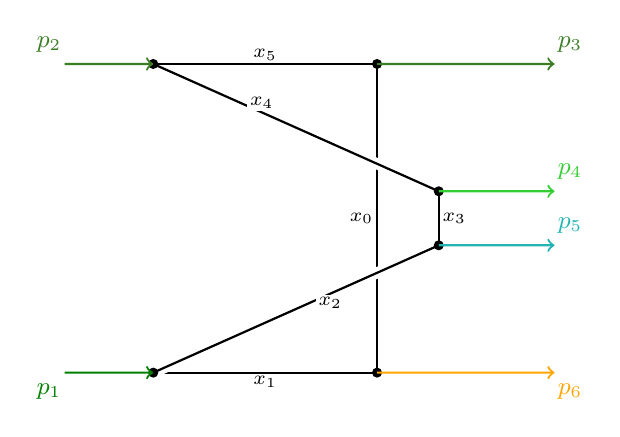
\begin{tikzpicture}[scale=.98]
 % The vertical placement displays the rapidity ordering
 % p3 >> (p4,p5) >> p6, while the top and bottom chains make the two
 % spacelike-collinear pairs manifest.
 \coordinate (v4) at (-2.20,2.00);
 \coordinate (v5) at ( .70,2.00);
 \coordinate (v3) at (1.50,.35);
 \coordinate (v2) at (1.50,-.35);
 \coordinate (v6) at ( .70,-2.00);
 \coordinate (v1) at (-2.20,-2.00);

 \draw[hrf internal] (v5)--node[hrf edge label,pos=.50,left] {$x_0$}(v6);
 \draw[hrf internal] (v6)--node[hrf edge label,pos=.50,below] {$x_1$}(v1);
 \draw[white,line width=4pt] (v1)--(v2);
 \draw[hrf internal] (v1)--node[hrf edge label,pos=.62,below] {$x_2$}(v2);
 \draw[hrf internal] (v2)--node[hrf edge label,pos=.50,right] {$x_3$}(v3);
 \draw[white,line width=4pt] (v3)--(v4);
 \draw[hrf internal] (v3)--node[hrf edge label,pos=.62,above] {$x_4$}(v4);
 \draw[hrf internal] (v4)--node[hrf edge label,pos=.50,above] {$x_5$}(v5);
 \foreach \v in {1,...,6} \node[hrf vertex] at (v\v) {};

 \draw[->,thick,OliveGreen] (-3.35,2.00)--(v4);
 \draw[->,thick,Green] (-3.35,-2.00)--(v1);
 \draw[->,thick,OliveGreen] (v5)--(3.00,2.00);
 \draw[->,thick,LimeGreen] (v3)--(3.00,.35);
 \draw[->,thick,TealBlue] (v2)--(3.00,-.35);
 \draw[->,thick,Orange] (v6)--(3.00,-2.00);
 \node[hrf leg label,text=OliveGreen] at (-3.55,2.25) {$p_2$};
 \node[hrf leg label,text=Green] at (-3.55,-2.25) {$p_1$};
 \node[hrf leg label,text=OliveGreen] at (3.20,2.25) {$p_3$};
 \node[hrf leg label,text=LimeGreen] at (3.20,.60) {$p_4$};
 \node[hrf leg label,text=TealBlue] at (3.20,-.10) {$p_5$};
 \node[hrf leg label,text=Orange] at (3.20,-2.25) {$p_6$};
\end{tikzpicture}
\caption{The common one-loop hexagon used for the NMRK and DSC analyses.
The nearly straight upper chain \(p_2\!-\!x_5\!-\!p_3\) and lower chain
\(p_1\!-\!x_1\!-\!p_6\) display the two spacelike-collinear pairs.  On the
right, the vertical separations display the rapidity ordering
\(p_3\gg(p_4,p_5)\gg p_6\); the relative order of \(p_4,p_5\) is immaterial
in NMRK.  The two crossings are deliberate and are not additional vertices.
This physical attachment ordering supports the HR (and associated Regge cut),
in contrast to the genuinely planar ordering \(123456\) with all four
emissions on one side.}
\label{fig:one-loop-hexagon}
\end{figure}

with \(\mathcal U=x_0+x_1+x_2+x_3+x_4+x_5\).  The full graph polynomial is
the same in both limits; only the invariant substitution changes.

In each case the cancelling monomials occur at different fixed-parameter
orders.  Thus \(\mathcal F_0\) does not contain the relevant cancellation
sector.  A face vector \(f\) first performs asymptotic-order alignment and
selects \(\mathcal F_\star=\mathcal F^{[f]}\).  Because
\(f\) and \(f+c\boldsymbol1\) select the same face, this discovery vector is
not yet the physical region vector.  The full occupied layer structure and
\(\mathcal U\) must fix the uniform component.

\subsection{Two-loop topology test and possible Regge-cut interpretation}

The two nearly horizontal chains in Fig.~\ref{fig:one-loop-hexagon} are the
\((23)\) and \((16)\) collinear sectors.  A \(t\)-channel exchange is an
internal path connecting these two chains.  The two central emissions
\(p_4,p_5\) may occur on the same such path or on two separate paths.
This distinction becomes explicit in the two-loop graphs used in the NMRK
and DSC audits.  With the external attachments of
Eq.~\eqref{eq:hexagon-edge-map}, their internal edges, in
\(x_0,\ldots,x_8\) order, are
\begin{align}
 E_{\rm PH}={}&\{(5,6),(1,8),(8,6),(1,2),(2,3),
                   (3,4),(4,7),(7,5),(7,8)\},\nonumber\\
 E_{\rm NPH}={}&\{(5,8),(1,8),(1,2),(2,3),(7,3),
                   (7,5),(4,7),(6,8),(4,6)\},\nonumber\\
 E_{\rm HP}={}&\{(5,6),(1,8),(8,6),(1,3),(3,4),
                   (4,7),(7,5),(7,2),(8,2)\}.
 \label{eq:two-loop-six-point-edges}
\end{align}

\begin{figure}[htbp]
\centering
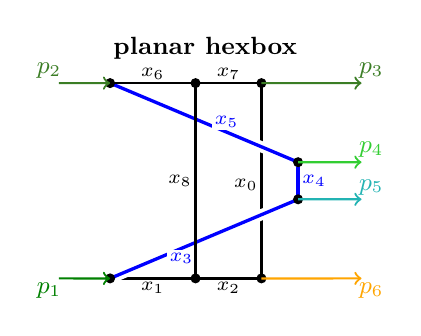
\begin{tikzpicture}[scale=.62]
 \coordinate (v4) at (-2.20,2.00);
 \coordinate (v7) at (-.45,2.00);
 \coordinate (v5) at ( .90,2.00);
 \coordinate (v3) at (1.65,.38);
 \coordinate (v2) at (1.65,-.38);
 \coordinate (v6) at ( .90,-2.00);
 \coordinate (v8) at (-.45,-2.00);
 \coordinate (v1) at (-2.20,-2.00);
 \node[font=\small\bfseries] at (-.25,2.72) {planar hexbox};

 \draw[hrf internal] (v5)--node[hrf edge label,pos=.52,left] {$x_0$}(v6);
 \draw[hrf internal] (v1)--node[hrf edge label,pos=.50,below] {$x_1$}(v8);
 \draw[hrf internal] (v8)--node[hrf edge label,pos=.50,below] {$x_2$}(v6);
 \draw[white,line width=4pt] (v1)--(v2);
 \draw[hrf internal,very thick,blue] (v1)--
   node[hrf edge label,pos=.38,below,text=blue] {$x_3$}(v2);
 \draw[hrf internal,very thick,blue] (v2)--
   node[hrf edge label,pos=.50,right,text=blue] {$x_4$}(v3);
 \draw[white,line width=4pt] (v3)--(v4);
 \draw[hrf internal,very thick,blue] (v3)--
   node[hrf edge label,pos=.38,above,text=blue] {$x_5$}(v4);
 \draw[hrf internal] (v4)--node[hrf edge label,pos=.50,above] {$x_6$}(v7);
 \draw[hrf internal] (v7)--node[hrf edge label,pos=.50,above] {$x_7$}(v5);
 \draw[hrf internal] (v7)--node[hrf edge label,pos=.50,left] {$x_8$}(v8);
 \foreach \v in {1,...,8} \node[hrf vertex] at (v\v) {};
 \draw[->,thick,OliveGreen] (-3.25,2)--(v4);
 \draw[->,thick,Green] (-3.25,-2)--(v1);
 \draw[->,thick,OliveGreen] (v5)--(2.95,2);
 \draw[->,thick,LimeGreen] (v3)--(2.95,.38);
 \draw[->,thick,TealBlue] (v2)--(2.95,-.38);
 \draw[->,thick,Orange] (v6)--(2.95,-2);
 \node[hrf leg label,text=OliveGreen] at (-3.45,2.25) {$p_2$};
 \node[hrf leg label,text=Green] at (-3.45,-2.25) {$p_1$};
 \node[hrf leg label,text=OliveGreen] at (3.15,2.25) {$p_3$};
 \node[hrf leg label,text=LimeGreen] at (3.15,.63) {$p_4$};
 \node[hrf leg label,text=TealBlue] at (3.15,-.13) {$p_5$};
 \node[hrf leg label,text=Orange] at (3.15,-2.25) {$p_6$};
\end{tikzpicture}
\hspace{5mm}
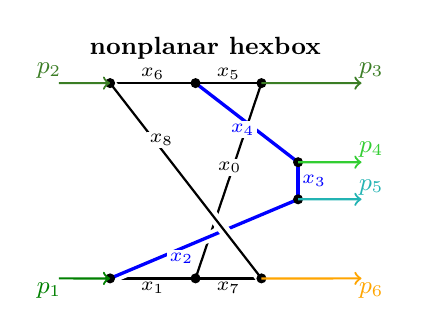
\begin{tikzpicture}[scale=.62]
 \coordinate (v4) at (-2.20,2.00);
 \coordinate (v7) at (-.45,2.00);
 \coordinate (v5) at ( .90,2.00);
 \coordinate (v3) at (1.65,.38);
 \coordinate (v2) at (1.65,-.38);
 \coordinate (v6) at ( .90,-2.00);
 \coordinate (v8) at (-.45,-2.00);
 \coordinate (v1) at (-2.20,-2.00);
 \node[font=\small\bfseries] at (-.25,2.72) {nonplanar hexbox};

 \draw[hrf internal] (v5)--node[hrf edge label,pos=.48,above] {$x_0$}(v8);
 \draw[hrf internal] (v1)--node[hrf edge label,pos=.50,below] {$x_1$}(v8);
 \draw[white,line width=4pt] (v1)--(v2);
 \draw[hrf internal,very thick,blue] (v1)--
   node[hrf edge label,pos=.38,below,text=blue] {$x_2$}(v2);
 \draw[hrf internal,very thick,blue] (v2)--
   node[hrf edge label,pos=.50,right,text=blue] {$x_3$}(v3);
 \draw[hrf internal,very thick,blue] (v3)--
   node[hrf edge label,pos=.54,below,text=blue] {$x_4$}(v7);
 \draw[hrf internal] (v7)--node[hrf edge label,pos=.50,above] {$x_5$}(v5);
 \draw[hrf internal] (v4)--node[hrf edge label,pos=.50,above] {$x_6$}(v7);
 \draw[hrf internal] (v8)--node[hrf edge label,pos=.50,below] {$x_7$}(v6);
 \draw[white,line width=4pt] (v4)--(v6);
 \draw[hrf internal] (v4)--node[hrf edge label,pos=.34,above] {$x_8$}(v6);
 \foreach \v in {1,...,8} \node[hrf vertex] at (v\v) {};
 \draw[->,thick,OliveGreen] (-3.25,2)--(v4);
 \draw[->,thick,Green] (-3.25,-2)--(v1);
 \draw[->,thick,OliveGreen] (v5)--(2.95,2);
 \draw[->,thick,LimeGreen] (v3)--(2.95,.38);
 \draw[->,thick,TealBlue] (v2)--(2.95,-.38);
 \draw[->,thick,Orange] (v6)--(2.95,-2);
 \node[hrf leg label,text=OliveGreen] at (-3.45,2.25) {$p_2$};
 \node[hrf leg label,text=Green] at (-3.45,-2.25) {$p_1$};
 \node[hrf leg label,text=OliveGreen] at (3.15,2.25) {$p_3$};
 \node[hrf leg label,text=LimeGreen] at (3.15,.63) {$p_4$};
 \node[hrf leg label,text=TealBlue] at (3.15,-.13) {$p_5$};
 \node[hrf leg label,text=Orange] at (3.15,-2.25) {$p_6$};
\end{tikzpicture}

\vspace{3mm}
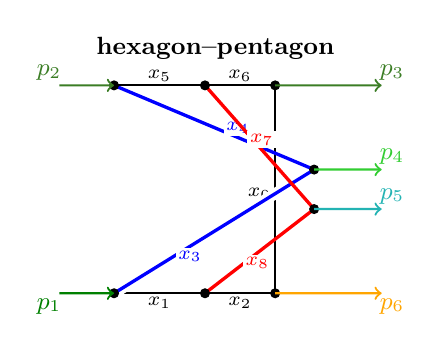
\begin{tikzpicture}[scale=.66]
 \coordinate (v4) at (-2.20,2.00);
 \coordinate (v7) at (-.45,2.00);
 \coordinate (v5) at ( .90,2.00);
 \coordinate (v3) at (1.65,.38);
 \coordinate (v2) at (1.65,-.38);
 \coordinate (v6) at ( .90,-2.00);
 \coordinate (v8) at (-.45,-2.00);
 \coordinate (v1) at (-2.20,-2.00);
 \node[font=\small\bfseries] at (-.25,2.72) {hexagon--pentagon};

 \draw[hrf internal] (v5)--node[hrf edge label,pos=.52,left] {$x_0$}(v6);
 \draw[hrf internal] (v1)--node[hrf edge label,pos=.50,below] {$x_1$}(v8);
 \draw[hrf internal] (v8)--node[hrf edge label,pos=.50,below] {$x_2$}(v6);
 \draw[white,line width=4pt] (v1)--(v3);
 \draw[hrf internal,very thick,blue] (v1)--
   node[hrf edge label,pos=.38,below,text=blue] {$x_3$}(v3);
 \draw[hrf internal,very thick,blue] (v3)--
   node[hrf edge label,pos=.38,above,text=blue] {$x_4$}(v4);
 \draw[hrf internal] (v4)--node[hrf edge label,pos=.50,above] {$x_5$}(v7);
 \draw[hrf internal] (v7)--node[hrf edge label,pos=.50,above] {$x_6$}(v5);
 \draw[hrf internal,very thick,red] (v7)--
   node[hrf edge label,pos=.52,above,text=red] {$x_7$}(v2);
 \draw[hrf internal,very thick,red] (v2)--
   node[hrf edge label,pos=.52,below,text=red] {$x_8$}(v8);
 \foreach \v in {1,...,8} \node[hrf vertex] at (v\v) {};
 \draw[->,thick,OliveGreen] (-3.25,2)--(v4);
 \draw[->,thick,Green] (-3.25,-2)--(v1);
 \draw[->,thick,OliveGreen] (v5)--(2.95,2);
 \draw[->,thick,LimeGreen] (v3)--(2.95,.38);
 \draw[->,thick,TealBlue] (v2)--(2.95,-.38);
 \draw[->,thick,Orange] (v6)--(2.95,-2);
 \node[hrf leg label,text=OliveGreen] at (-3.45,2.25) {$p_2$};
 \node[hrf leg label,text=Green] at (-3.45,-2.25) {$p_1$};
 \node[hrf leg label,text=OliveGreen] at (3.15,2.25) {$p_3$};
 \node[hrf leg label,text=LimeGreen] at (3.15,.63) {$p_4$};
 \node[hrf leg label,text=TealBlue] at (3.15,-.13) {$p_5$};
 \node[hrf leg label,text=Orange] at (3.15,-2.25) {$p_6$};
\end{tikzpicture}
\caption{The two-loop graphs in the same rapidity-ordered embedding as
Fig.~\ref{fig:one-loop-hexagon}.  The upper and lower horizontal chains are
the \((23)\) and \((16)\) collinear sectors.  In each hexbox, the single blue
\(t\)-channel path carries both central emissions.  In the
hexagon--pentagon, \(p_4\) lies on the blue path and \(p_5\) on the distinct
red path.  Crossings without black dots are not vertices.}
\label{fig:two-loop-six-point-graphs}
\end{figure}

The current certificates give
\begin{center}
\small
\begin{tabular}{@{}lccc@{}}
\toprule
Graph & central-emission paths & NMRK with \(w=z\) & generic DSC\\
\midrule
one-loop hexagon & same & 1 full certificate & 1 full certificate\\
planar hexbox & same & 7 full \(+\) 4 boundary & 1 full certificate\\
nonplanar hexbox & same & 1 full \(+\) 2 boundary & no certificate\\
hexagon--pentagon & separate & no staged candidate & no staged candidate\\
\bottomrule
\end{tabular}
\end{center}
These entries count certified vectors, not necessarily distinct physical
regions.  Within the tested NMRK set, however, the same-exchange graphs have
an HR and the separate-exchange graph does not.  This is evidence for a
topology criterion, not yet a theorem; the DSC nonplanar-hexbox result also
shows that the topology is not sufficient in every kinematic expansion.

The crossed ordering is the six-point Mandelstam region in which Regge-cut
effects arise.  Bartels' reggeon calculus organized high-energy amplitudes
by one- and two-reggeon states in successive \(t\)-channels
\cite{Bartels1980}.  Bartels, Lipatov and Sabio Vera later showed that, for
six and more legs, the BDS ansatz is incompatible with the Regge cuts
predicted by the BFKL approach in appropriate physical channels
\cite{BartelsLipatovSabioVera2008a}, and computed the leading-logarithmic
color-octet cut contribution and the corresponding \(2\to4\) and \(3\to3\)
discontinuities \cite{BartelsLipatovSabioVera2008b}.
That correction is the high-energy contribution that must reside in the
six-point BDS remainder function, and it initiated the extensive subsequent
study of remainder functions in multi-Regge kinematics.

It is therefore natural to conjecture that the HR found here is the
parameter-space origin of the relevant \(t\)-channel cut.  This connection
is not established by the present certificates alone.  It requires matching
the local positive pinch and its region integral to the appropriate
Mandelstam discontinuity and multi-reggeon exchange.  Enlarging the topology
sample in Fig.~\ref{fig:two-loop-six-point-graphs} is a direct way to test
the conjecture.

\subsection{NMRK with the additional surface \texorpdfstring{\(w=z\)}{w=z}}

Use the MSLCV chart
\begin{equation}
 X_{34}=\frac{\widehat X_{34}}{\eta},\qquad
 X_{56}=\frac{\widehat X_{56}}{\eta},\qquad
 X_{45},Q,z,\bar z,w,\bar w=O(1),\qquad \eta\to0^+,
 \label{eq:nmrk-scaling-example}
\end{equation}
with
\begin{equation}
 Q,\widehat X_{34},X_{45},\widehat X_{56},K_z>0,\qquad
 K_z=(1-z)(1-\bar z)>0.
 \label{eq:nmrk-domain-example}
\end{equation}
On this physical NMRK sheet \(z,\bar z\) and \(w,\bar w\) are conjugate
pairs.  The restriction \(w=z\), \(\bar w=\bar z\) is additional to NMRK.
For generic NMRK the relevant bilinear determinant is proportional to
\((w-z)(\bar w-\bar z)\), so the HR is absent.

On the restricted surface define
\begin{equation}
 L_1^N=(1+X_{45})x_4-\widehat X_{34}X_{45}x_5,\qquad
 L_2^N=(1+X_{45})x_2-K_zX_{45}\widehat X_{56}x_1.
 \label{eq:nmrk-factors-example}
\end{equation}
The selected face has
\begin{equation}
 \mathcal F_\star^N=\FSL^N+\FObs^N
 =\SLcolour{Q\widehat X_{34}\widehat X_{56}L_1^NL_2^N}+0.
 \label{eq:nmrk-decomposition-example}
\end{equation}
The discovery data and certified answer are
\begin{align}
 f_N&=(-1,-1,-2,-1,-2,-1),&
 h_N&=(-1,-1,-1,-1,-1,-1),\nonumber\\
 \vHR^N&=(-2,-2,-3,-2,-3,-2;1),&
 (\WSL,\WHR)&=(-4,-3).
 \label{eq:nmrk-vector-example}
\end{align}
There is no intermediate cancellation layer.  At \(\WHR\),
\begin{align}
 \mathcal U_{-3}&=\HRcolour{x_2+x_4},\nonumber\\
 \mathcal F_{-3}&=\HRcolour{-Q\widehat X_{34}X_{45}\widehat X_{56}
 (K_zx_0x_2+K_zx_0x_4+\widehat X_{34}x_3x_5
 +K_z\widehat X_{56}x_1x_3)}.
 \label{eq:nmrk-WHR-example}
\end{align}
These monomials give a unique lower facet directly.  The required new
capability is asymptotic-order alignment itself; once the correct face is
exposed, the cancellation has depth one.

\subsection{Generic double spacelike-collinear kinematics}

For DSC let \(\varepsilon\to0^+\) and use the real physical slice
\begin{equation}
 a<0,\qquad -1<\tau_1<0,\qquad \tau_2<-1,\qquad
 z_D<0,\qquad \bar z_D<0.
 \label{eq:dsc-domain-example}
\end{equation}
The symbols \(z_D,\bar z_D\) are conjugate on the standard real transverse
MRK branch, but after continuation to this DSC sheet they are two independent
real roots.  In the graph-polynomial sign convention the adjacent invariants
behave as
\begin{align}
 s_{12}&=-\frac{\tau_2}{a(1+\tau_1)(1+\tau_2)}+O(\varepsilon),&
 s_{23}&=\frac{\varepsilon^2\tau_1}{a\bar z_D}+O(\varepsilon^3),\nonumber\\
 s_{34}&=\frac{1}{(a-1)(1+\tau_2)}+O(\varepsilon),&
 s_{45}&=-\frac1a,\nonumber\\
 s_{56}&=\frac{\tau_1}{(a-1)(1+\tau_1)}+O(\varepsilon),&
 s_{16}&=\frac{\varepsilon^2\tau_2z_D}{a}+O(\varepsilon^3).
 \label{eq:dsc-invariants-example}
\end{align}
Thus \(s_{23},s_{16}<0\), while \(s_{12},s_{34},s_{45},s_{56}>0\), as
required for \(2\to4\) scattering with legs 1 and 2 incoming.

The cancellation factors and selected-face decomposition are
\begin{align}
 L_1^D&=(1+\tau_2)x_4+x_5,&
 L_2^D&=\tau_1x_1+(1+\tau_1)x_2,
 \label{eq:dsc-factors-example}\\
 \mathcal F_\star^D&=\FSL^D+\FObs^D
 =\SLcolour{-(a-1)a^2\bar z_D^{,2}L_1^DL_2^D}+0.
 \label{eq:dsc-decomposition-example}
\end{align}
Both factors have positive zeros,
\begin{equation}
 x_5=-(1+\tau_2)x_4>0,\qquad
 x_2=-\frac{\tau_1}{1+\tau_1}x_1>0.
 \label{eq:dsc-positive-pinch-example}
\end{equation}
For crossed double-timelike collinear splittings \(\tau_i>0\), so these
same factors have one sign for positive \(x_i\) and the pinch disappears.

The discovery vectors are
\begin{equation}
 f_D=(-2,-2,-2,-1,-2,-2),\qquad
 h_D=(-1,-1,-1,-1,-1,-1).
 \label{eq:dsc-discovery-vectors}
\end{equation}
Their naive sum is not the answer.  With
\(\ideal_D=\langle L_1^D,L_2^D\rangle\), the actual occupied layers obey
\begin{equation}
 \underbrace{\SLcolour{\mathcal F_{-4}\in\ideal_D^2}}_{
  \operatorname{ord}_{\ideal_D}=2}
 \; +\;
 \underbrace{\Othercolour{\mathcal F_{-3}\in\ideal_D\setminus\ideal_D^2}}_{
  \operatorname{ord}_{\ideal_D}=1}
 \; +\;
 \underbrace{\HRcolour{\mathcal F_{-2}\notin\ideal_D}}_{
  \operatorname{ord}_{\ideal_D}=0}.
 \label{eq:dsc-two-layer-colours}
\end{equation}
The middle layer contains 52 nonzero terms.  It is not a missing power of
\(\varepsilon\): it vanishes to first order on the common pinch.  The leading
\(\mathcal U\) layer is
\begin{equation}
 \mathcal U_{-2}=\HRcolour{x_0+x_1+x_2+x_4+x_5},
 \label{eq:dsc-U-leading}
\end{equation}
and the full ideal-jet balance gives
\begin{equation}
 \vHR^D=(-2,-2,-2,0,-2,-2;1),
 \qquad (\WSL,\WHR)=(-4,-2),
 \label{eq:dsc-vector-example}
\end{equation}
with gap two.  A local dissection pulls back to this same vector.

This example is why asymptotic-order alignment cannot be treated as a
cosmetic preprocessing step.  HRF must (i) expose the cancelling face,
(ii) retain every occupied layer, (iii) compute successive ideal orders,
and (iv) use the first nonvanishing LP layer to fix the uniform ambiguity of
the face representative.  Simply adding \(f_D+h_D\) would give the wrong
total vector and the wrong cancellation depth.

\subsection{What the two limits share---and what they do not}

After their separate kinematic rescalings, the factor coefficients are
identified by
\begin{equation}
 \frac{K_zX_{45}\widehat X_{56}}{1+X_{45}}
 =-\frac{\tau_1}{1+\tau_1},
 \qquad
 \frac{\widehat X_{34}X_{45}}{1+X_{45}}
 =-\frac{1}{1+\tau_2}.
 \label{eq:composite-factor-map}
\end{equation}
Hence the two order-aligned \(\FSL\) supports describe the same type of
positive cancellation hypersurface.  The next layers differ:
\begin{center}
\begin{tabular}{@{}lccc@{}}
\toprule
Expansion & certified \(\boldsymbol v\) & \((\WSL,\WHR)\) & depth\\
\midrule
NMRK with \(w=z\) & \((-2,-2,-3,-2,-3,-2)\) & \((-4,-3)\) & 1\\
generic DSC & \((-2,-2,-2,0,-2,-2)\) & \((-4,-2)\) & 2\\
\bottomrule
\end{tabular}
\end{center}
The common generator does not make the two limits identical.  The first
resolved LP layer, and therefore the physical region vector, remembers the
path by which the singular hypersurface is approached.

\section{What the examples teach}

\begin{center}
\small
\begin{tabular}{@{}>{\raggedright\arraybackslash}p{0.22\textwidth}
                    >{\raggedright\arraybackslash}p{0.26\textwidth}
                    >{\raggedright\arraybackslash}p{0.44\textwidth}@{}}
\toprule
Family & New structure & Capability needed not to miss the HR\\
\midrule
Crown & simultaneous positive cancellation, \(\FObs=0\) & keep a
multi-equation positive pinch and determine its uniform scaling\\
Crown descendants & contraction-minor boundary regions & scan boundary
strata and compare restricted ideals, not only parent interiors\\
Five-point seed & \(\FObs\ne0\), non-uniform scaling & isolate \(\FSL\)
before imposing the positive pinch; retain the obstruction\\
Vertex correction & primitive non-binomial factor & generate and test
general polynomial ideals rather than monomial pairs only\\
NMRK, \(w=z\) & cancellation on a nontrivial asymptotic face & align
orders before running the ordinary HRF construction\\
DSC & a second occupied cancellation layer & resolve the ideal filtration
and fix the uniform face ambiguity from the full LP polynomial\\
\bottomrule
\end{tabular}
\end{center}

The progression is cumulative.  Later examples require the earlier tests in
addition to their new feature.  In every case the final statement is again
geometric: after cancellation is resolved, the leading polynomial must be a
lower facet in coordinates adapted to the pinch.  HRF reconstructs the
coefficient and Landau information absent from the original Newton polytope;
it does not replace lower-facet certification.

Allowing massive internal propagators would relax the standing massless
multiaffinity assumption.  The resulting quadratic edge-parameter dependence
changes the possible cancellation jets and the local facet problem.  It is a
genuine extension of this framework, not another example in the present
tour.

\appendix
\section{Notation summary}

\begin{center}
\begin{tabular}{@{}p{0.38\textwidth}p{0.57\textwidth}@{}}
\toprule
Symbol & Meaning\\
\midrule
\(\delta\) & kinematic expansion parameter\\
\(\s\) & real kinematic coordinates; their physical domain \(\K\) is specified
  by explicit inequalities\\
\(x_e\) & independent LP edge parameter, integrated over \((0,\infty)\)\\
\(\mathcal C_{\rm LP}=\mathbb R_{>0}^{N}\) & non-projective LP integration
  contour\\
\(\mathcal P=\mathcal U+\mathcal F\) & Lee--Pomeransky polynomial\\
\(\deg_x\mathcal U=L,\ \deg_x\mathcal F=L+1\) & massless graph-polynomial
  degrees; both polynomials are linear in each individual \(x_e\)\\
\(\widehat{\mathcal P}=\mathcal F+x_0\mathcal U\) & optional homogeneous
  \((N+1)\)-parameter embedding\\
\(m_i=c_i(\s)\delta^{a_i}\x^{\boldsymbol r_i}\) & monomial of
  \(\mathcal P\)\\
\(\boldsymbol r_i\) & length-\(N\) LP-parameter exponent vector of \(m_i\)\\
\(\vec r_i=(\boldsymbol r_i;a_i)\) & augmented exponent point\\
\(\mathcal F_0\) & strict fixed-\(\x\) leading polynomial\\
\(\mathcal F^{[\phi]}\) & face selected by the preliminary alignment vector
  \(\boldsymbol\phi\)\\
\(\mathcal F_\star\) & HRF starting polynomial, either
  \(\mathcal F_0\) or \(\mathcal F^{[\phi]}\)\\
\(\SSL\) & superleading monomial support selected by the scaling law\\
\(\FSL\) & superleading cancellation sector\\
\(\FObs\) & obstruction polynomial\\
\(f_j\) & non-monomial cancellation factor\\
\(\ideal\) & ideal of independent cancellation factors at the common pinch\\
\(\boldsymbol\rho\) & relative scaling obtained on a selected face\\
\(\vHR=(\boldsymbol v_{\HR};1)\) & certified total hidden-region vector\\
\(\WSL\) & common individual weight of SL monomials\\
\(\WHR\) & first resolved nonvanishing LP weight after cancellation\\
\(\WHR-\WSL\) & cancellation depth\\
\SLcolour{red terms} & individually superleading sector at \(\WSL\)\\
\HRcolour{blue terms} & resolved physical leading layer at \(\WHR\)\\
\Othercolour{black terms} & all other layers, including intermediate
  ideal-valued cancellations\\
\bottomrule
\end{tabular}
\end{center}

\begin{thebibliography}{99}

\bibitem{LeePomeransky2013}
R.~N.~Lee and A.~A.~Pomeransky,
\emph{Critical points and number of master integrals},
JHEP \textbf{11} (2013) 165,
\href{https://arxiv.org/abs/1308.6676}{arXiv:1308.6676}.

\bibitem{PakSmirnov2011}
A.~Pak and A.~V.~Smirnov,
\emph{Geometric approach to asymptotic expansion of Feynman integrals},
Eur.\ Phys.\ J.\ C \textbf{71} (2011) 1626,
\href{https://arxiv.org/abs/1011.4863}{arXiv:1011.4863}.

\bibitem{JantzenSmirnovSmirnov2012}
B.~Jantzen, A.~V.~Smirnov and V.~A.~Smirnov,
\emph{Expansion by regions: revealing potential and Glauber regions
automatically},
Eur.\ Phys.\ J.\ C \textbf{72} (2012) 2139,
\href{https://arxiv.org/abs/1206.0546}{arXiv:1206.0546}.

\bibitem{GardiEtAl2024}
E.~Gardi, F.~Herzog, S.~Jones and Y.~Ma,
\emph{Dissecting polytopes: Landau singularities and asymptotic expansions
in \(2\to2\) scattering},
\href{https://arxiv.org/abs/2407.13738}{arXiv:2407.13738}.

\bibitem{GardiEtAl2026}
E.~Gardi et al.,
\emph{Spacelike-Collinear Scattering by the Method of Regions},
\href{https://arxiv.org/abs/2607.15126}{arXiv:2607.15126}.

\bibitem{Bartels1980}
J.~Bartels,
\emph{High-energy behavior in a non-Abelian gauge theory. II. First
corrections to \(T_{n\to m}\) beyond the leading \(\ln s\) approximation},
Nucl.\ Phys.\ B \textbf{175} (1980) 365--401,
\href{https://doi.org/10.1016/0550-3213(80)90019-X}
{doi:10.1016/0550-3213(80)90019-X}.

\bibitem{BartelsLipatovSabioVera2008a}
J.~Bartels, L.~N.~Lipatov and A.~Sabio Vera,
\emph{BFKL Pomeron, Reggeized gluons and Bern--Dixon--Smirnov amplitudes},
Phys.\ Rev.\ D \textbf{80} (2009) 045002,
\href{https://arxiv.org/abs/0802.2065}{arXiv:0802.2065}.

\bibitem{BartelsLipatovSabioVera2008b}
J.~Bartels, L.~N.~Lipatov and A.~Sabio Vera,
\emph{\(\mathcal N=4\) supersymmetric Yang--Mills scattering amplitudes at
high energies: the Regge cut contribution},
Eur.\ Phys.\ J.\ C \textbf{65} (2010) 587--605,
\href{https://arxiv.org/abs/0807.0894}{arXiv:0807.0894}.

\end{thebibliography}

\end{document}
